\section{Recurrent Neural Network}

Die bisher betrachteten Neuralen Netzwerke gehören zu den \emph{forwärtsgekoppelten} Netzwerken (engl. \emph{Feedforward Networks}). Dieser Begriff bezieht sich darauf, dass die Eingangssignale ohne Bezug auf vorherige Durchläufe ein Ergebnis generieren. Das RNN besitzt dagegen eine solche Verbindung zwischen den Neuronen derselben Schicht oder Verbindungen von Neuronen zu Neuronen einer vorgegebenen Schicht. In Abbildung \ref{rnnAufbau} ist zu sehen wie so etwas aussehen könnte. 

\begin{figure}[!htb]
	\centering
	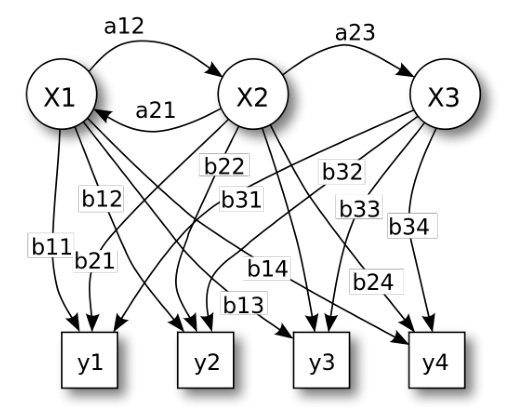
\includegraphics[width=.6\linewidth]{./img/rnn_aufbau}
	\mycaption{RNN - Aufbau}{ss}
	\label{fig:rnnAufbau}
\end{figure} 


RNNs lernen ähnlich wie die bisherigen Netzwerke mit dem wesentlichen Zusatz, dass sie Wissen aus früheren Iterationen \emph{erinnern} während sie den aktuellen Output generieren. In anderen Worten: Sie bekommen sowohl Eingangssignale durch den Trainingsdatensatz sowie von sich selbst durch Rückkopplungen während der Ausführung selbst. Deshalb ist die Reihenfolge in der bestimmte Eingaben in das Netzwerk gespeist werden von Bedeutung. 

Diese Struktur wird in vielen unterschiedlichen Bereichen genutzt. Besonders gut eignet sie sich jedoch um bestimmte Muster zu ergänzen aber auch bei der Mustererkennung im Bereich der Sprachanalyse stellt dies ein wertvolles Werkzeug dar. 
